% Overview of assurance argument structure
The high-level structure of our CASE assurance pattern is inspired by the D-MILS argument pattern~\cite{dmils}, in which system dependability properties are assured via modules arguing component, compositional, and implementation correctness.  
Although verifying functional, safety, and other dependability properties is necessary for a comprehensive system assurance case, the CASE pattern presented here only addresses cyber-resiliency.  The intention is for the resulting assurance argument to be integrated into a full system assurance case, if necessary.

The high-level CASE argument structure is depicted in Figure~\ref{fig:top-level}, with the top-level goal being ``The system is acceptably cyber-resilient".  
This goal is then substantiated by arguments that cyber-resiliency requirements have been appropriately identified and then satisfied, both in the system model and the \textit{realization} of the system model as a built, deployable system.

\begin{figure}[h] 
	\centering 
	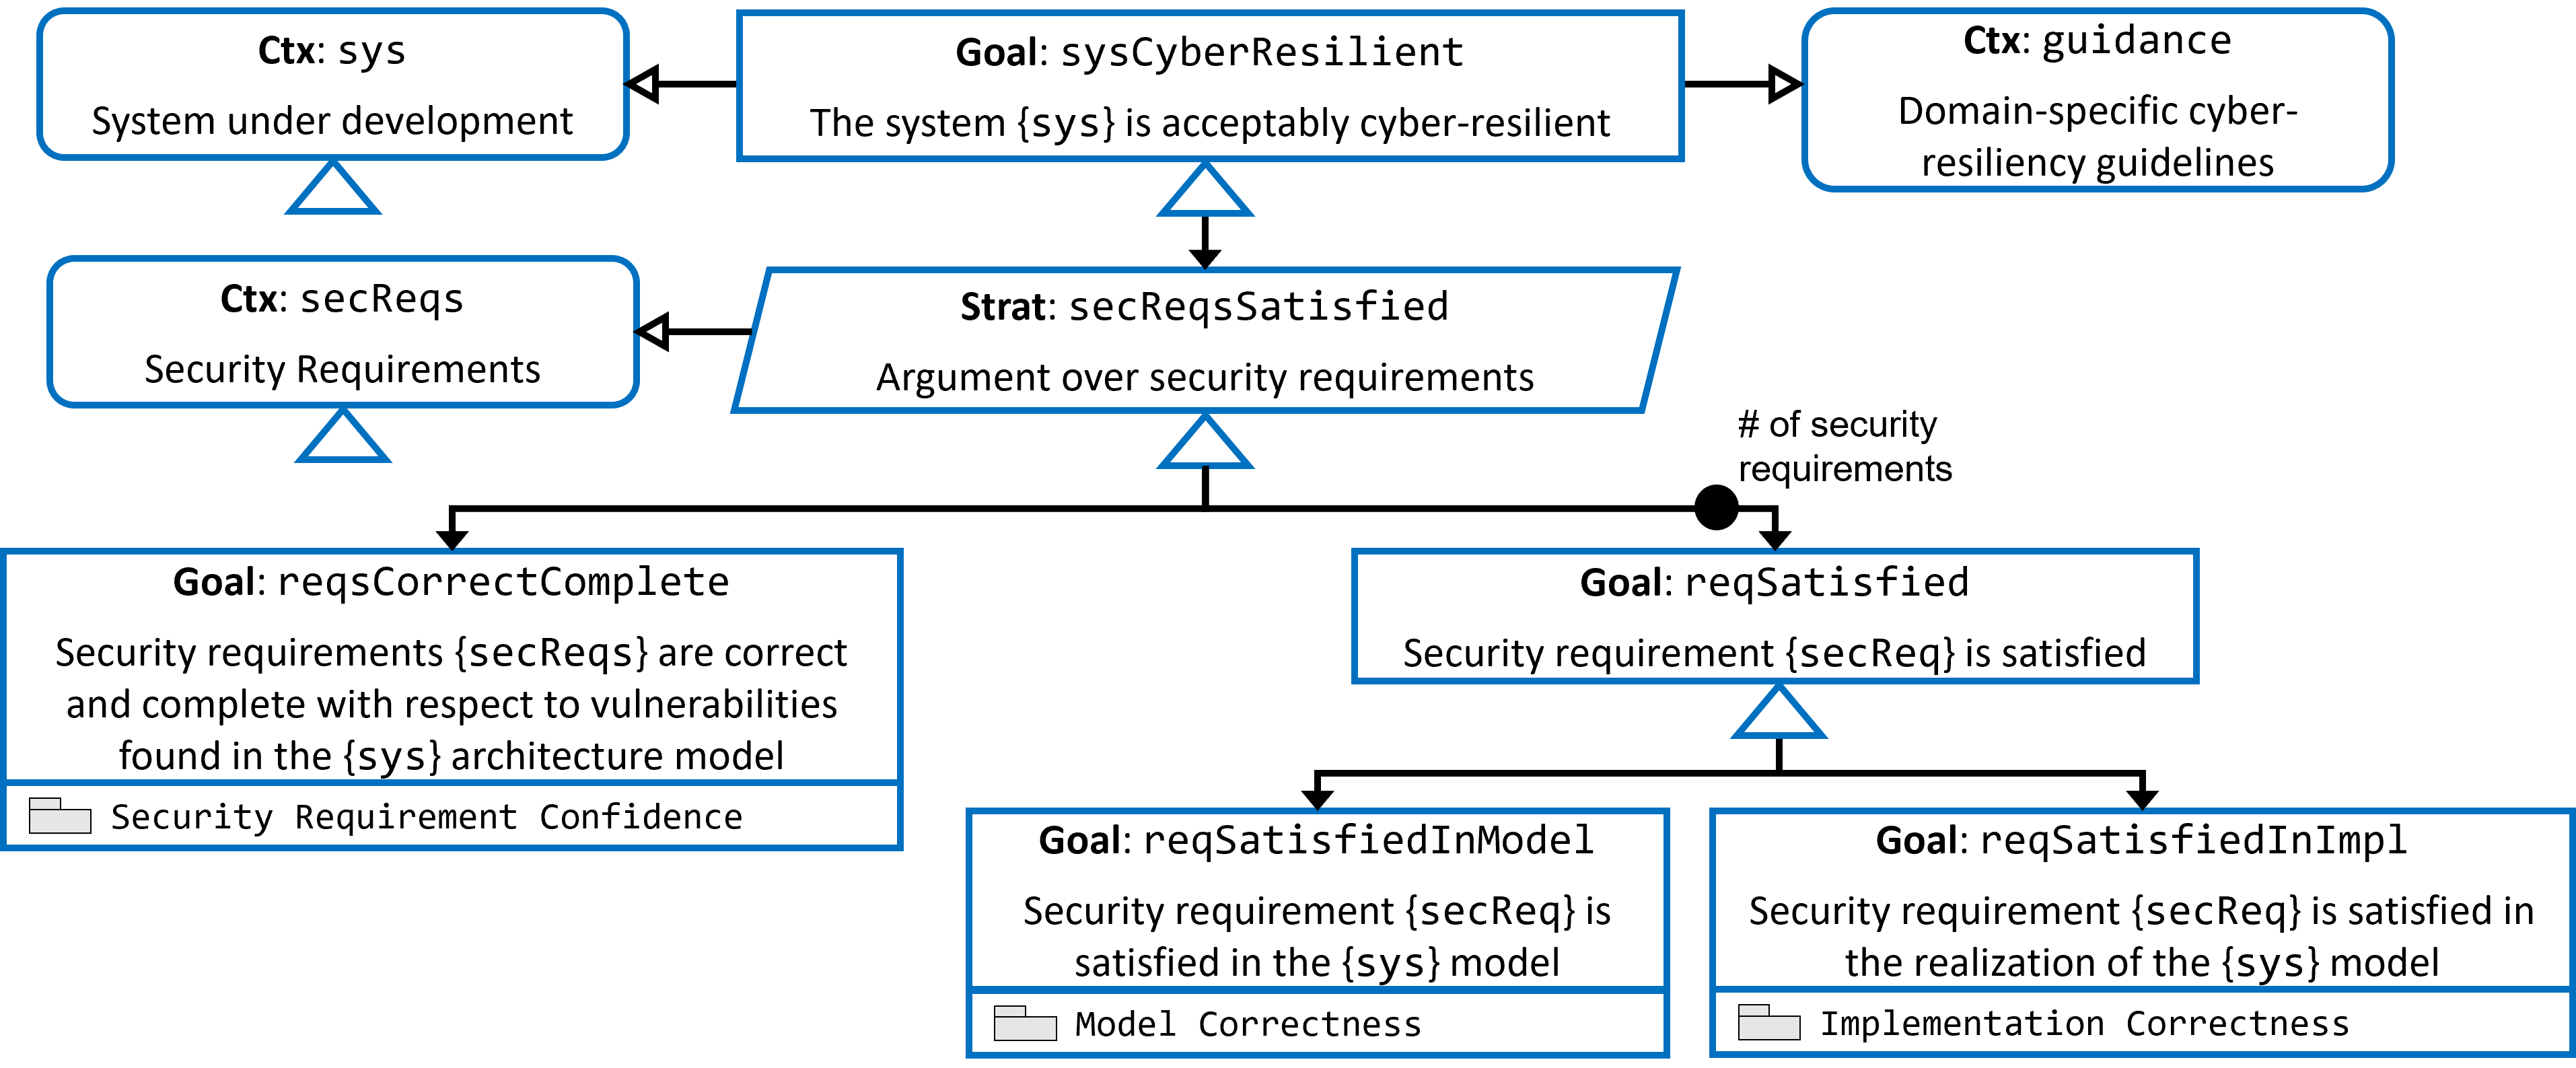
\includegraphics[width=\textwidth]{figs/top-level.png}
	\caption{Top-level assurance pattern structure.}
	\label{fig:top-level} 
\end{figure}


% Describe at a high-level how each workflow step should be assured.  Refer to figure.  Then dive into BriefCASE assurance pattern.

% Security requirements are correct and complete
\subsection{Cyber Requirement Correctness and Completeness}
BriefCASE currently includes two cybersecurity plug-ins, GearCASE~\cite{gearcase2020} and DCRYPPS~\cite{dcrypps2019}, that analyze an AADL model and output a set of cyber requirements corresponding to vulnerabilities detected in the model.  
BriefCASE maintains the generated requirements within the framework as assurance goals using the Resolute tool~\cite{resolute2014}.  
In addition to providing an AADL annex grammar for representing assurance cases, Resolute includes an evaluation engine for determining whether sufficient evidence exists (both internal and external to the AADL workspace) to support assurance claims.  
Because BriefCASE manages the development artifacts associated with the CASE workflow, it automatically provides Resolute with instructions on how those artifacts can be used to support specific cyber-resiliency goals.
%Resolute generates assurance arguments in a tree format, but also supports export to graphical tools such as AdvoCATE~\cite{advocate}.  


The assurance argument for cybersecurity requirement correctness and completeness is shown in Figure~\ref{fig:req-correct-complete}.  
%
In the figure, it can be seen that in order to support the requirement correctness and completeness claim, we must provide evidence that the full set of cyber requirements passed through a review process, were imported into the BriefCASE environment as Resolute goals or omitted with rationale, and that successive analyses on updated versions of the model finds no new vulnerabilities.  The latter reflects the iterative step in the workflow (depicted by the left-pointing arrow in Figure~\ref{fig:workflow}), in which a modified model must be re-analyzed after applying a mitigation for a previously generated requirement.  This is necessary in order to demonstrate that the mitigation of one vulnerability does not inadvertently introduce other vulnerabilities.  To argue that the current model was analyzed appropriately, we must be able to demonstrate that the model is well-formed; that is, it complies with modeling guidelines, that the analysis was indeed performed on the current version of the model, and that the analysis does not produce any new applicable requirements.

\begin{figure}[h] 
	\centering 
	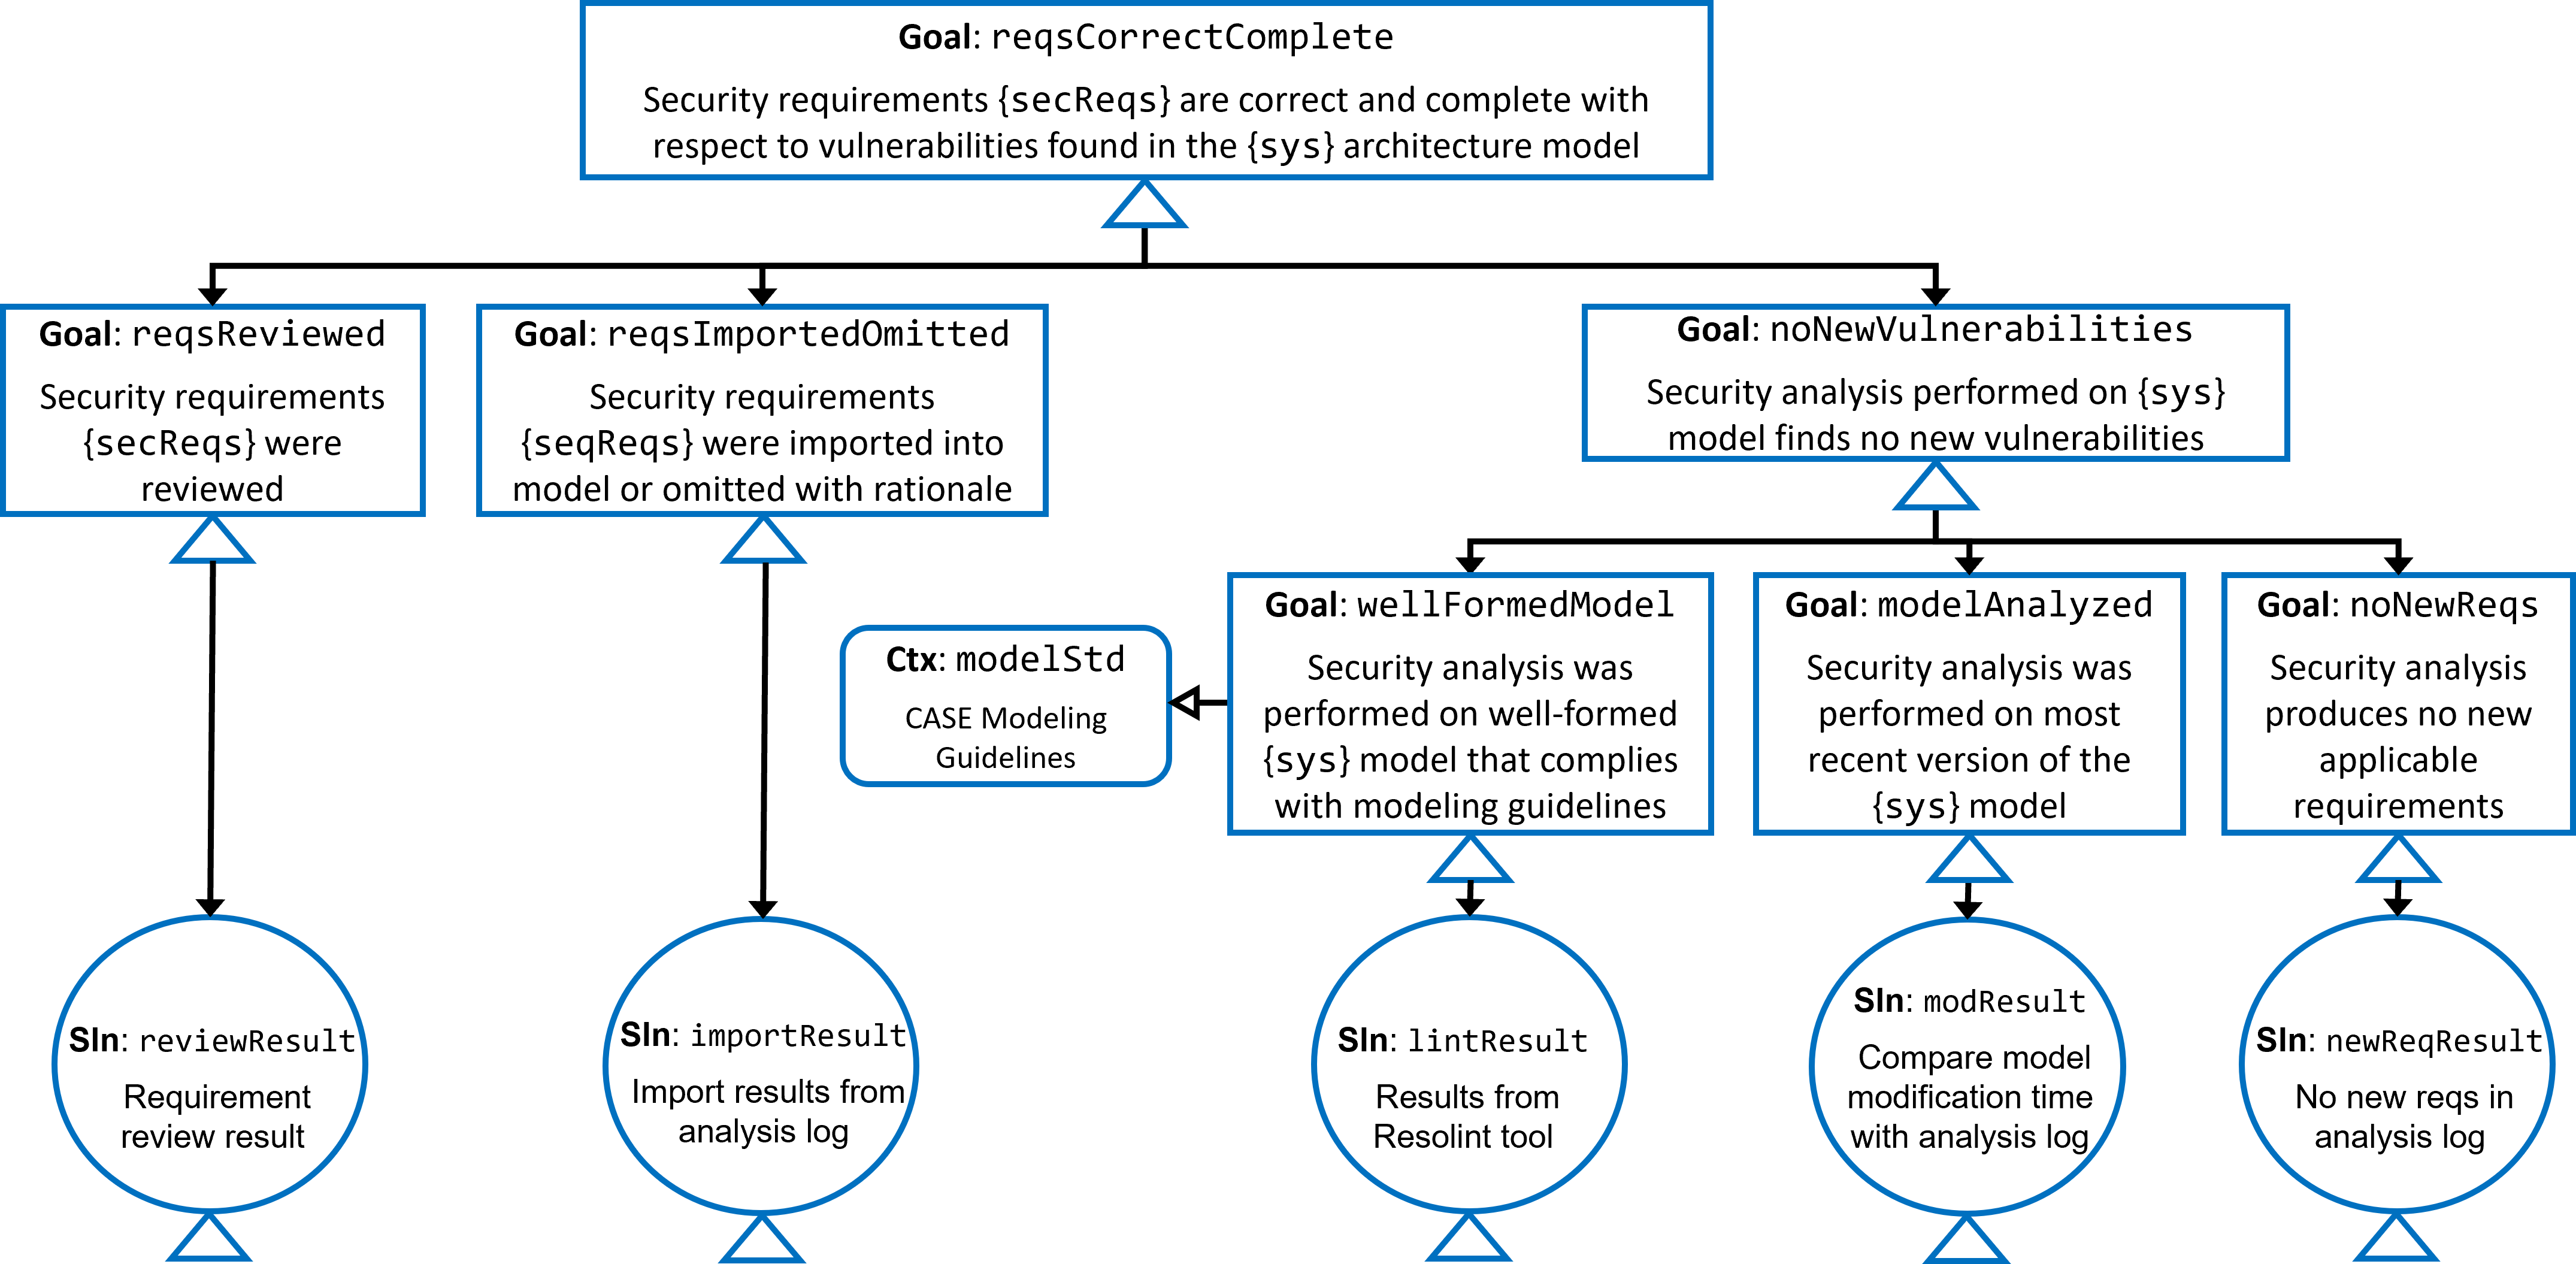
\includegraphics[width=\textwidth]{figs/req-correct-complete.png}
	\caption{Assurance pattern for security requirement correctness and completeness.}
	\label{fig:req-correct-complete} 
\end{figure}

% Model assurance
\subsection{Cyber Requirements are Satisfied in the System Model}
BriefCASE includes a library of automated model transformations corresponding to common cyber requirement classes.  Each transformation modifies the model to harden it against a specific vulnerability, thereby mitigating the associated threat and addressing the driving requirement.  In addition, the transformations automatically update the corresponding Resolute goals with instructions that enable Resolute to evaluate whether the goal is supported by the necessary evidence.

% NOT SURE HOW MUCH SPACE WE WILL HAVE HERE.
% USE FILTER AS EXAMPLE
% OTHERWISE, JUST REFERENCE DESTION PAPER 
Because the transformations modify the architecture model in different ways, assuring that a specific requirement is satisfied in the model will be argued according to a transformation-specific pattern.  For example, a message well-formedness requirement on a component's input port can be addressed by inserting a filter on the communication channel upstream of the target component.  The corresponding assurance pattern for this mitigation is shown in Figure~\ref{fig:filter}.

\begin{figure}[h] 
	\centering 
	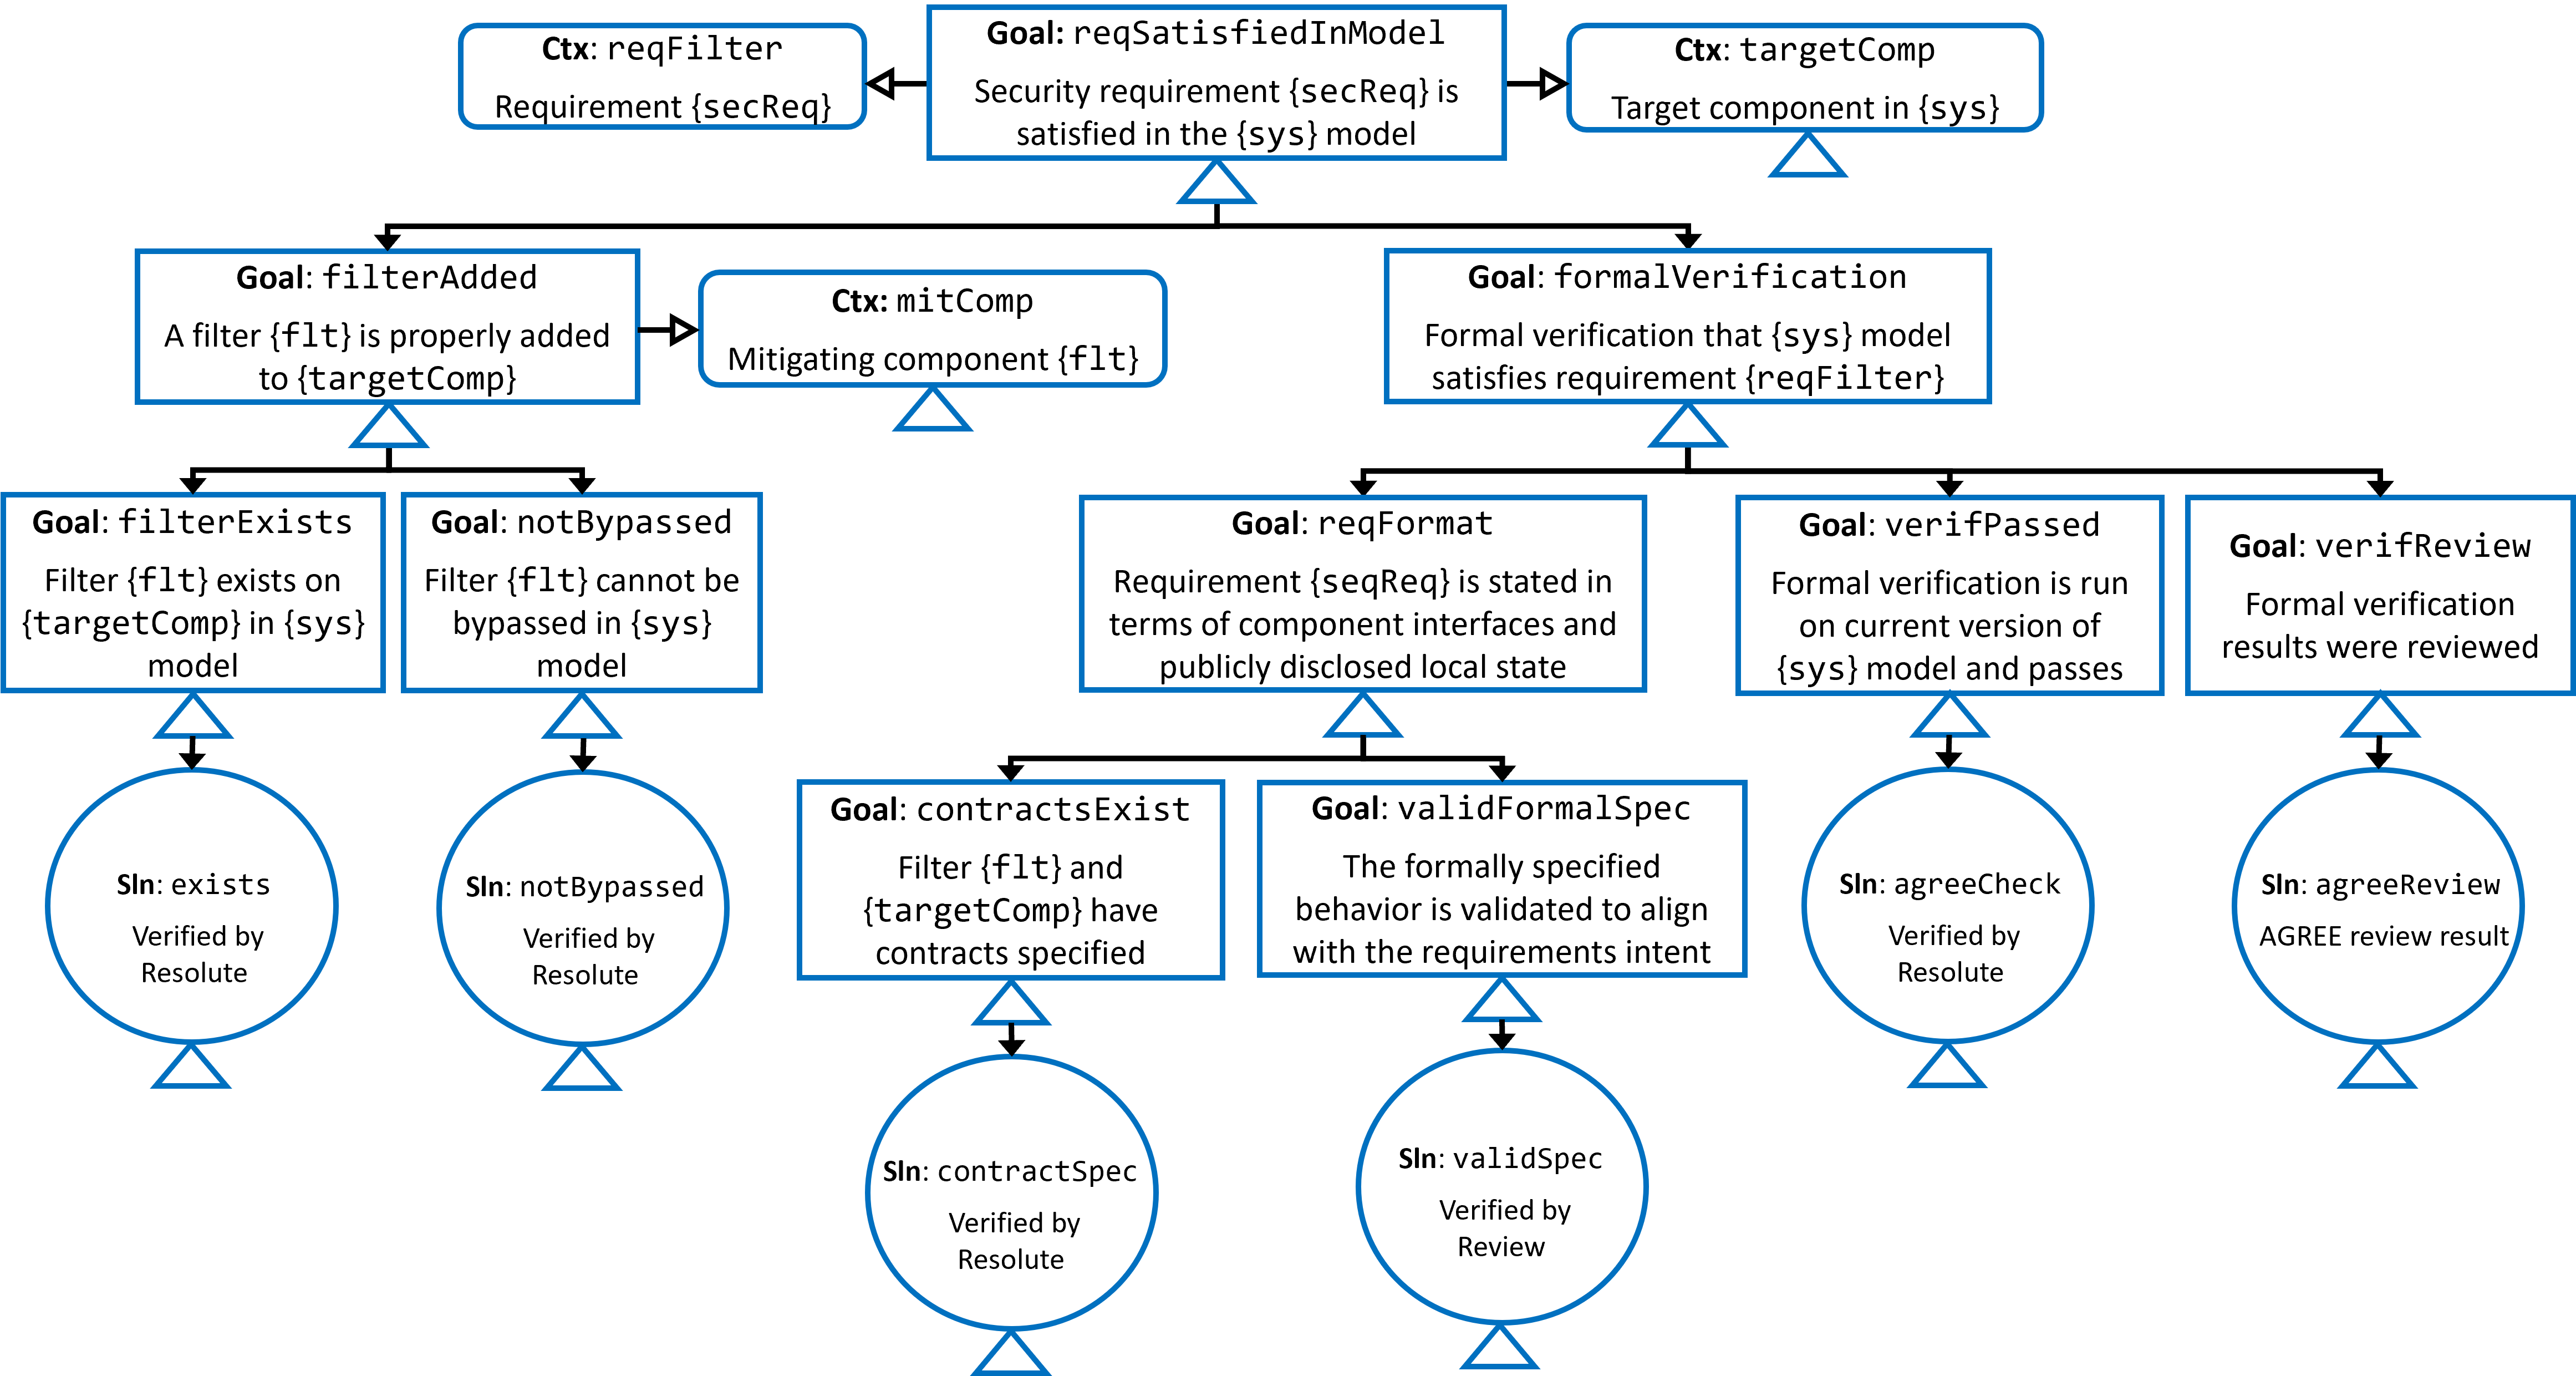
\includegraphics[width=\textwidth]{figs/filter.png}
	\caption{Assurance pattern for a filter mitigation.}
	\label{fig:filter} 
\end{figure}

% Implementation assurance
\subsection{Cyber Requirements are Satisfied in the Realization of the Model}
% Where BriefCASE implementations can come from (legacy/manual implementation, SPLAT synthesis, pre-packaged - Attestation, seL4, HAMR)

In the CASE workflow, a software component implementation could have various origins.  It could be legacy, third-party, or manually implemented code. It could also be generated from an external behavioral model such as Simulink or be synthesized directly from the component's contract.  In BriefCASE, the latter is performed by the SPLAT tool~\cite{case-verified-filter}, which synthesizes the implementation of high-assurance components in the CakeML language~\cite{cakeml} directly from a formal assume-guarantee contract specified in the AADL component's AGREE annex~\cite{compositional-analysis-agree}.  In addition to providing a formally verified compiler, CakeML enables SPLAT to generate a proof of correctness that the synthesized implementation is correct with respect to the contract.

In addition to the software component application code, infrastructure code and the operating system itself must be implemented and integrated into a deployable system.  The HAMR~\cite{hamr} system build tool included with BriefCASE generates the infrastructure code, along with correspondence proofs that the intra-component connections specified in the model are maintained in the implementation, and that no new connections have been created.  This is made possible in part by building to an seL4~\cite{sel4-cacm18} target.  seL4 is a formally verified microkernel that provides time and space partitioning guarantees.  

The structure of the implementation branch of the assurance pattern therefore examines the provenance of the software and assures it ...

\begin{figure}[h] 
	\centering 
	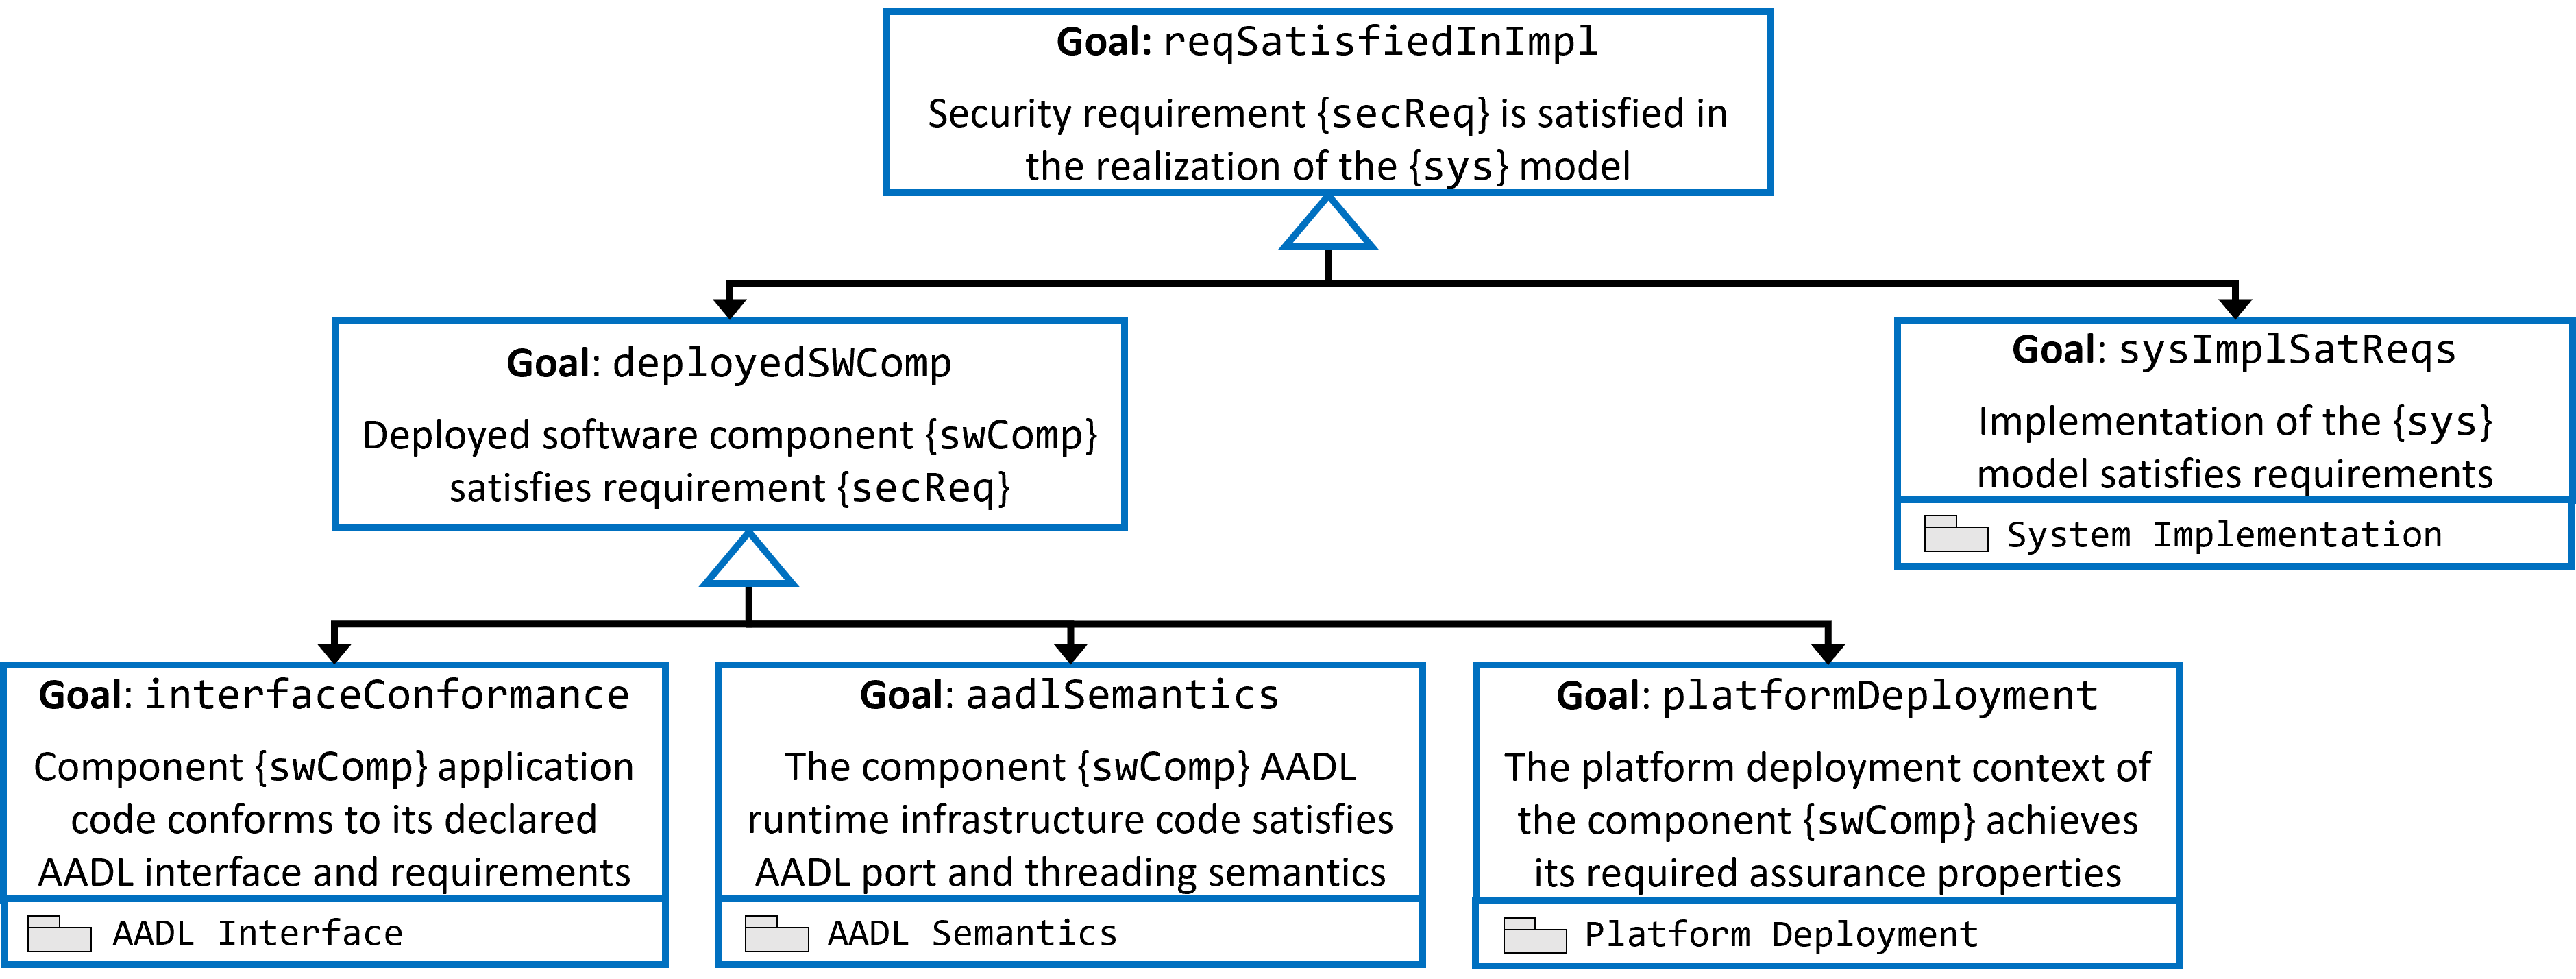
\includegraphics[width=\textwidth]{figs/req-satisfied-in-model-realization.png}
	\caption{Assurance pattern for arguing the requirement is satisfied in the realization of the model.}
	\label{fig:req-satisfied-in-model-realization} 
\end{figure}



\begin{figure}[h]
	\centering 
	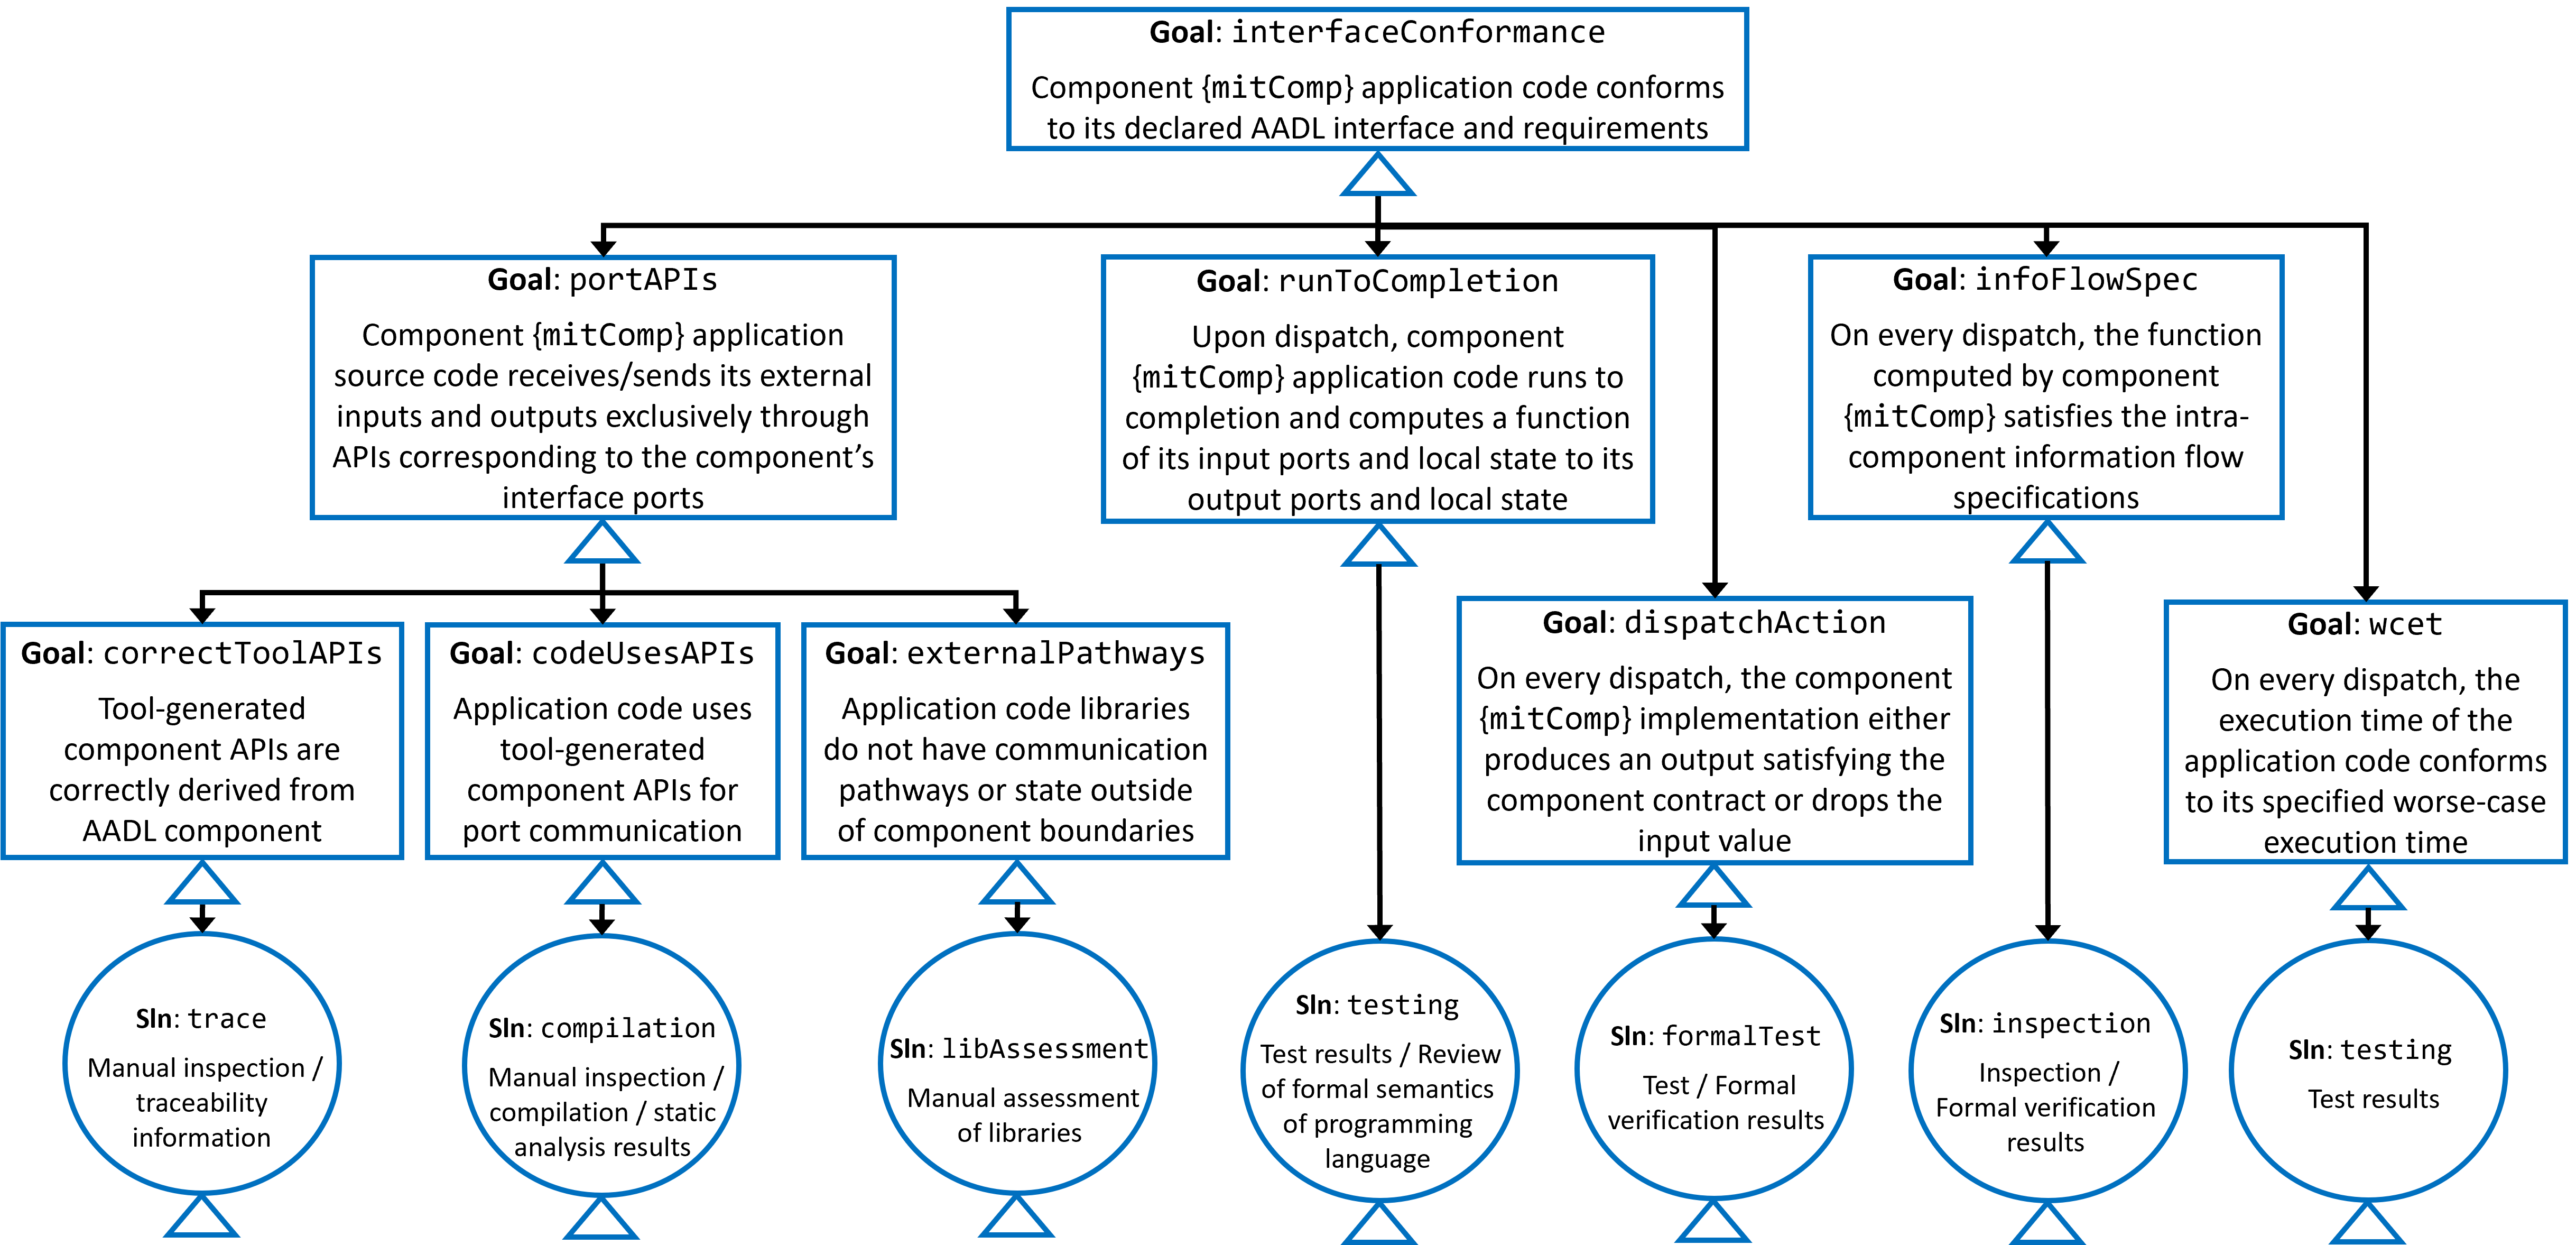
\includegraphics[width=\textwidth]{figs/code-conforms-to-interface-and-requirements.png}
	\caption{Assurance pattern for arguing component code conforms to the specified interface and requirements.}
	\label{fig:code-conforms-to-interface-and-requirements} 
\end{figure}


\begin{figure}[h] 
	\centering 
	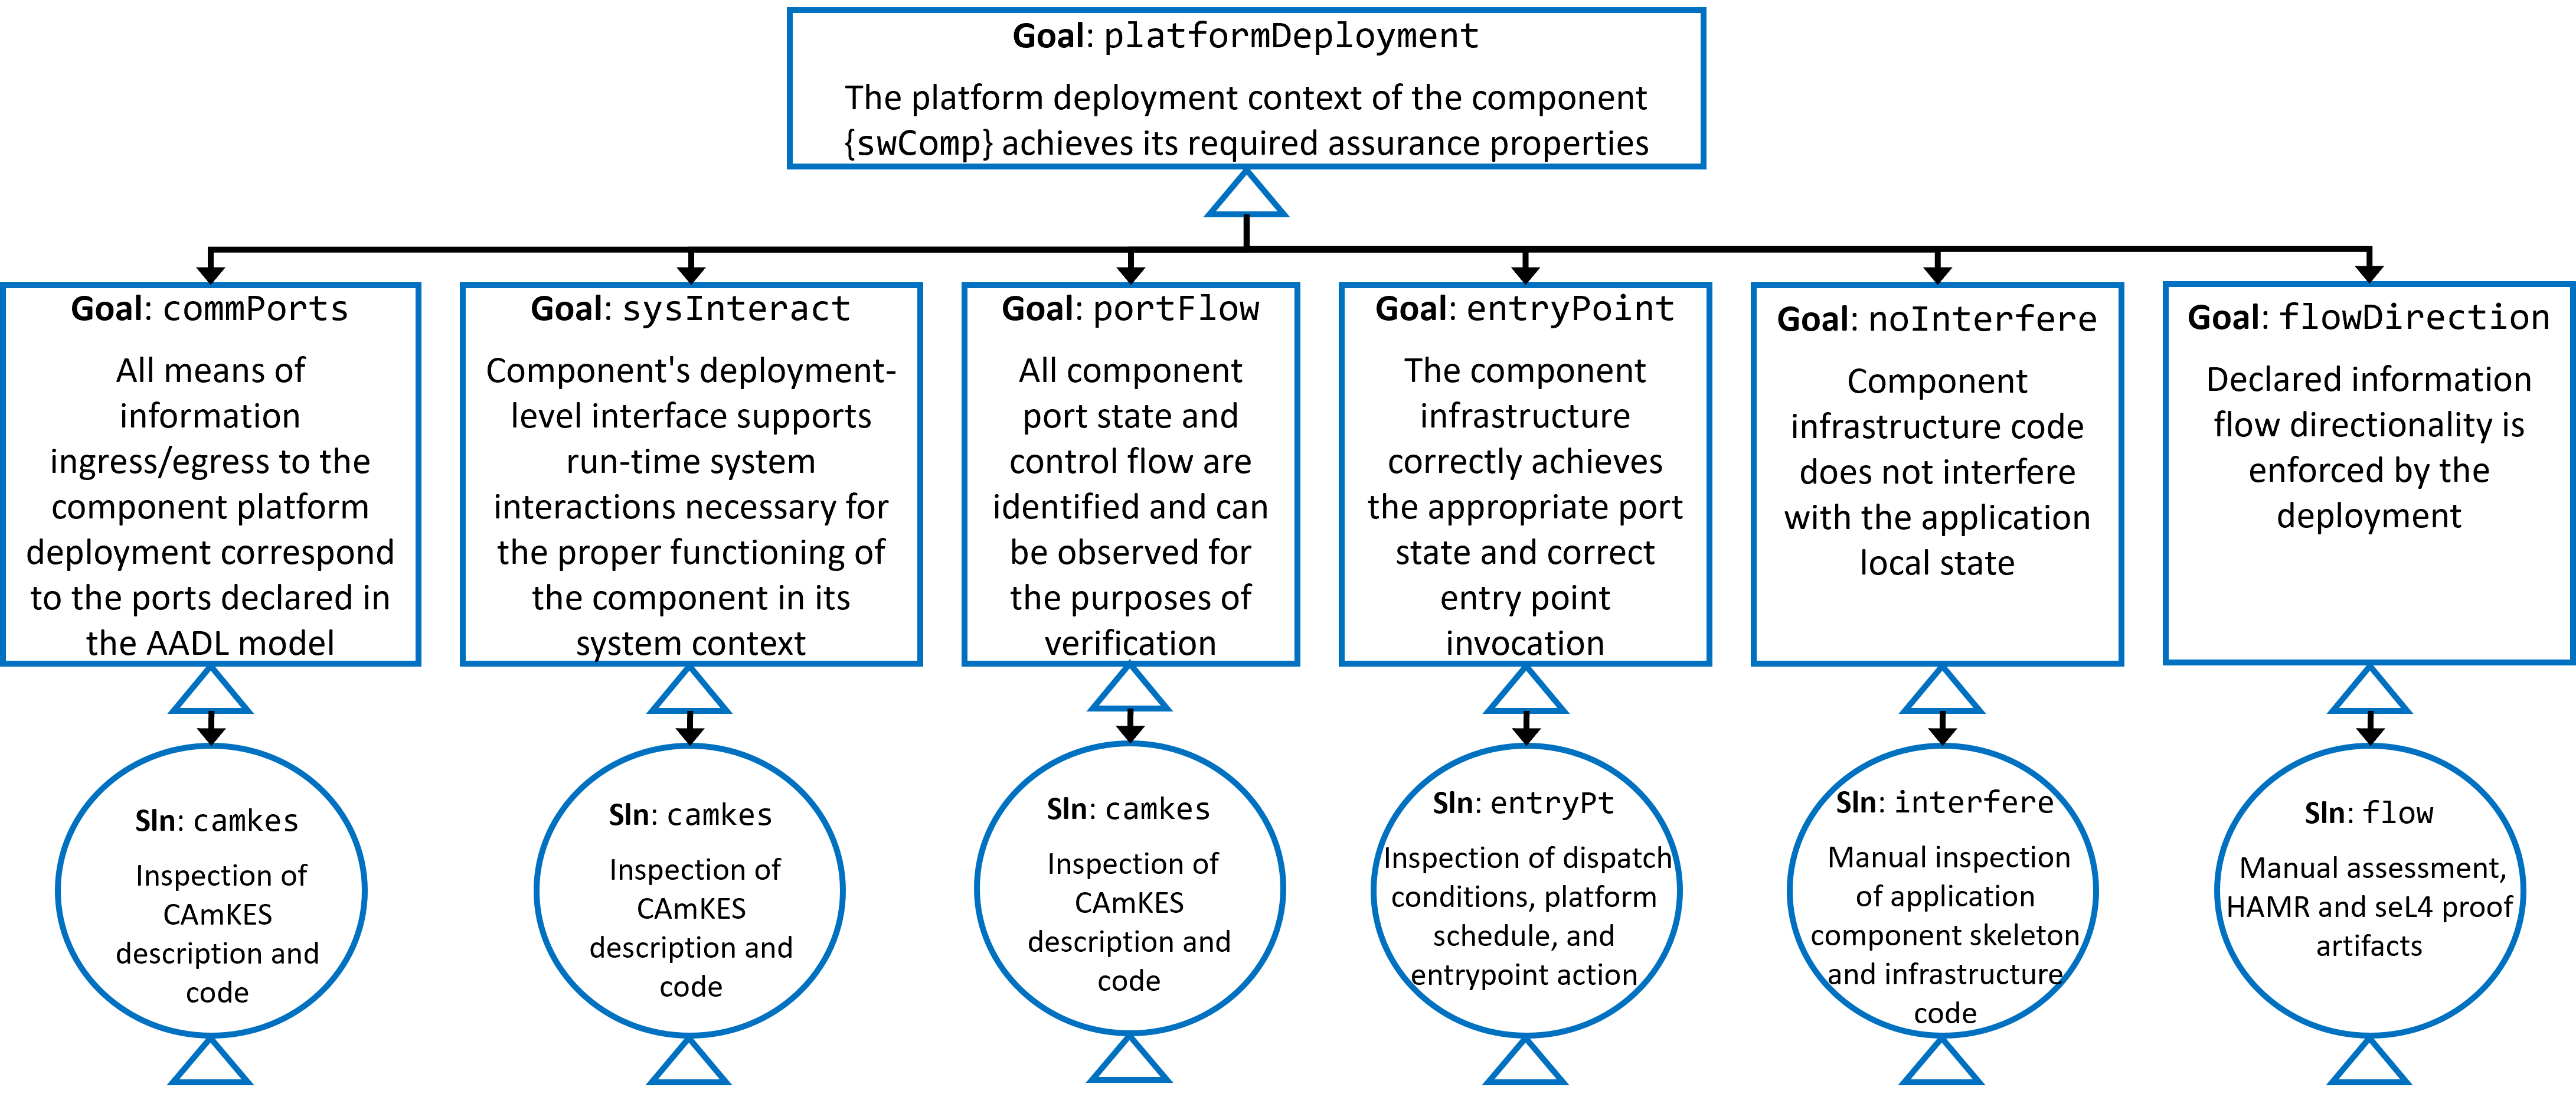
\includegraphics[width=\textwidth]{figs/platform-deployment-context-achieves-assurance-properties.png}
	\caption{Assurance pattern for arguing platform deployment context achieves the required assurance properties.}
	\label{fig:platform-deployment-context-achieves-assurance-properties} 
\end{figure}